\documentclass[11pt]{article}
\usepackage[small]{titlesec}
\usepackage[top = 0.66in,textwidth = 6.5in, textheight=9.1in]{geometry}

\usepackage{amsmath}
\usepackage{graphicx}
\usepackage{latexsym}
\usepackage{color}
\usepackage{amssymb}
\usepackage{tabularx}
\usepackage{fancyhdr}
\usepackage{verbatim}
\usepackage{multirow}
\usepackage{framed}
\usepackage{natbib}
\usepackage{float, subfig}
\usepackage{enumitem}
\usepackage{mathtools}
\usepackage{mathrsfs}
\usepackage{amsfonts}
\usepackage{listings}
\usepackage{amsthm}
\usepackage{grffile}
\usepackage{sidecap}
\usepackage{pbox}

\def\qed{\hfill{\(\vcenter{\hrule height1pt \hbox{\vrule width1pt height5pt
     \kern5pt \vrule width1pt} \hrule height1pt}\)} \medskip}

\newtheorem{theorem}{Theorem}
\newtheorem{lemma}[theorem]{Lemma}
\newtheorem{corollary}[theorem]{Corollary}
\newtheorem{proposition}[theorem]{Proposition}
\newtheorem{conjecture}[theorem]{Conjecture}
\newtheorem{remark}{Remark}
\newtheorem{example}{Example}
\renewcommand{\textfraction}{0.0}
\newcommand{\dst}{\displaystyle}
\newcommand{\minx}{\mbox{\( \dst \min_{x \in X} \)}}
\newcommand{\Efx}{\mbox{\( \dst E f (x, \xi) \)}}
\newcommand{\Efxhat}{\mbox{\( \dst E f (\hat{x}, \xi) \)}}
\newcommand{\hxx}{\mbox{\( \hat{x} \)}}
\newcommand{\bpi}{\bar{\pi}}
\newcommand{\xx}{\mbox{\( x \)}}
\newcommand{\txxi}{\mbox{\(\xi\)}}
\newcommand{\var}{\mbox{var}}
\newcommand{\cF}{{\cal F}}
\newcommand{\cG}{{\cal G}}
\newcommand{\cN}{{\cal N}}
\newcommand{\cO}{{\cal O}}
\newcommand{\txi}{{\xi}}
\newcommand{\PP}{\mbox{\(SP\)}}
\newcommand{\PPn}{\mbox{\(SP_n\)}}
\newcommand{\PPnx}{\mbox{\(SP_{n_x}\)}}
\newcommand{\noi}{\noindent}
\renewcommand{\ss}{\smallskip}
\newcommand{\ms}{\medskip}
\newcommand{\bs}{\bigskip}
\newcommand{\st}{\mbox{s.t.}}
\newcommand{\wpo}{\mbox{wp1}}
\newcommand{\iid}{\mbox{i.i.d.\ }}
\newcommand{\vsmo}{\vspace*{-0.1in}}
\newcommand{\vsmt}{\vspace*{-0.2in}}
\newcommand{\vso}{\vspace*{0.1in}}
\newcommand{\vst}{\vspace*{0.2in}}
\newcommand{\mc}{\multicolumn}
\newcommand{\cP}{{\cal P}}
\newcommand{\underv}{\mbox{$\underbar{$v$}$}}
%\allowdisplaybreaks 

\renewcommand{\P}{{\mathbb P}}
\newcommand{\E}{{\mathbb E}}
\newcommand{\R}{{\mathbb R}}
\renewcommand{\Re}{{\mathbb R}}

\bibliographystyle{plain}

\begin{document}
%0.27
\baselineskip0.25in

\begin{center}
\begin{large}
\begin{bf}

A Report on Disruption Model \ms

Haoxiang Yang \ms

\today \ms
\end{bf}
\end{large}
\end{center}

\section{Introduction to a Disruption Model}
	In a sequential decision problem, we make decisions in a sequence of time periods, which may be under the influence of uncertainty. The uncertainty usually takes the form of an unknown outcome of parameters, which is not realized before making the decision. In stochastic programming, we model uncertainty by assuming the outcome is governed by a known distribution, or a stochastic process, and in robust optimization we instead assume the outcome belongs to an uncertainty set. Those models mainly focus on the magnitude of the uncertainty and %The distribution or the feasible region of parameters are fixed across the time horizon.}% 
	usually assume that the uncertainty exists in every single time period with the same known distribution or the same uncertainty set. However, it may not be the case in many real-world problems. Here, we model uncertainty in the time periods in which uncertainty occurs, focusing on the notion of disruptions in sequential decision problems. For our purposes, a disruption is a type of event under which uncertain parameters change in a significant way, in value, distribution, etc. We will view disruptions as events that occur infrequently, but that can have a significant impact. So, a disruption could be a one-time event, or an event that happens only a limited number of times over the planning horizon. There have been only limited number of literatures focused on this problem. There are a few papers (\cite{BGZ15},\cite{G78}) addressing the issue of non-stationary objective functions. \cite{RDM13} considers a probabilistic bicriteria model with disruption using stochastic programming. \cite{MSW09} has the closest setting to our problem as it gives a military application of modeling the attack as the disruption. Our work would like to generalize those results and gain some theoretical insights.

\section{A Stochastic Program for Modeling Disruptions}
	\subsection{Single-disruption Formulation}\label{1Dformulation}
	We begin by assuming that at most one disruption can occur over a fixed time horizon. The parameters before and after the disruption are fixed. Here \(\mathscr{T}=\{1,2,\dots,T\}\) represents the time horizon fixed for the sequential decision problem. For an infinite horizon problem, \(T=+\infty\).\\ %As the randomness is not stagewise independent, we can introduce state variable to the model \cite{S11}.
	\newline We assume the possible scenario lies in a finite scenario set \(\Omega\). The probability of each scenario is \(p^\omega\) and \(\sum_{\omega \in \Omega} p^\omega = 1\). The disruption happens at time period \(t_d^\omega\) under scenario \(\omega \in \Omega\), after the decision ot the time period \(t_d^\omega\) is made. We can consider the no-disruption scenario as an element in \(\Omega\) and denote it by \(\omega_0\).\\
	\newline We denote the variables at each epoch before the disruption as \(x_t \text{ and } s_t, t = 1 \dots T\). \(s\) contains the information of the actions/records before observing the uncertainty while \(x\) contains the information of the actions/records after observing the uncertainty in each period. We formulate the model in this structure because it will greatly reduce the complexity of the non-anticipative constraints. \\
	\newline Since there is a positive probability that the disruption may not occur in the timespan, \(x \text{ and } s\) has to be indexed by the whole timespan \(\mathscr{T}\). We denote the decision after the disruption as \(\overline{x_t^\omega} \text{ and } \overline{s_t^\omega}, t \in \{t_d^\omega, \dots, T\}\). There exists a connection between \(s_{t_d^\omega}\) and \(\overline{s_{t_d^\omega}^\omega}\) under scenario \(\omega\) to tie the process before the disruption and the process after the disruption.\\
	\newline Suppose there is no discount factor in this problem, and the problem has a linear objective function and linear constraints. We assume that two sequences of parameters \(CX_t, t\in \mathscr{T}\) and \(CS_t, t\in \mathscr{T}\) are known, which can describe the costs of variables before the disruption under all scenarios. Given a scenario \(\omega\), we assume that parameters \(\overline{CX_t^\omega} \text{ and } \overline{CS_t^\omega}, t \in \{t_d^\omega, \dots, T\}\) are also known to describe the objective function after the disruption. \\
	\newline It is easy to see that without the disruption, it is a deterministic linear programming problem. We can form an optimization model as follows. Notice that it is possible to have same matrix \(A, B, \text{ and } H\) for each period time, when the dynamic of the system does not change over time.
	% We need to write down a multi-stage stochastic optimization model first. Then we show the multi-stage one is equivalent to the one below.
	\begin{align}
		\min \quad & \sum_{\omega \in \Omega} p^\omega [\sum_{t = 1}^{t_d^\omega-1}{(CX_tx_t+CS_ts_t)}+\sum_{t = t_d^\omega}^{T}{(\overline{CX_t^\omega}\ \overline{x_t^\omega} + \overline{CS_t^\omega}\ \overline{s_t^\omega}}) ]\\
		\text{s.t.} \quad & A_{t-1}s_{t-1} + B_tx_{t} + H_ts_{t} = b_t & \quad & \forall t = 1 \dots T\\
		& \overline{A_{t-1}^\omega} \  \overline{s_{t-1}^\omega} + \overline{B_{t}^\omega}\ \overline{x_{t}^\omega} + \overline{H_{t}^\omega}\ \overline{s_{t}^\omega} = \overline{b_t^\omega}  & \quad & \forall t = t_d^\omega \dots T,\ \forall \omega \in \Omega\\
		& \overline{s_{t_d^\omega}^\omega} = s_{t_d^\omega}& \quad & \forall \omega \in \Omega\\
		& x_t, s_t \geq 0 & \quad & \forall t = 1 \dots T\\
		& \overline{x_t^\omega}, \overline{s_t^\omega} \geq 0 & \quad & \forall t = t_d^\omega \dots T,\ \forall \omega \in \Omega
	\end{align}
	Suppose in each epoch the disruption happens according to a Bernoulli distribution with some probability \(p_t\) if there has not been any disruption before. The disruption will lead the system to a deterministic path. The scenario tree is illustrated in Figure~\ref{scenarioTree}.
	\begin{figure}[H]
		\centering
		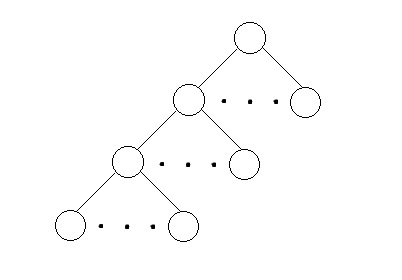
\includegraphics[width=0.6\textwidth]{single disruption model fig1}
		\caption{Single disruption model with 4 epochs}
		\label{scenarioTree}
	\end{figure}
	
	
	\subsection{L-shape Method}
	Given the formulation in Section~\ref{1Dformulation}, we could write down the original problem as a two-stage stochastic linear program. The first stage decision variables are \(x_t, s_t, \ \forall t = 1\dots T\) and the second stage could be viewed as functions of the first stage variables \(G^\omega(s_{t_d^\omega}), \ \forall \omega \in \Omega\).\\
	\newline The master problem can be formulated as follows:
	\begin{align}
		(M) \quad \min \quad & \sum_{\omega \in \Omega}p^\omega\sum_{t = 1}^{t_d^\omega - 1}(CX_t x_t + CS_t s_t) + \sum_{\omega \in \Omega} p^\omega \phi^\omega & \\
		\text{s.t.} \quad & A_{t-1}s_{t-1} + B_tx_{t} + H_ts_{t} = b_t \quad & \forall t = 1 \dots T\\
		& \hat{\pi}_k^\omega s_{t_d^\omega - 1} + \sum_{t = t_d^\omega}^T \gamma_{t,k}^\omega \overline{b_t^\omega} \leq 0 \quad & \forall \omega \in \Omega, \forall k = 1,2 \dots\\
		% Optimality cut generation
		& \phi^\omega \geq G^\omega(s_{t_d^\omega}^l) + \pi^\omega_l(s_{t_d^\omega - 1} - s_{t_d^\omega - 1}^l) \quad & \forall l = 1,2 \dots\\
		& x_t, s_t \geq 0 \quad & \forall t = 1 \dots T
	\end{align}
	\noindent The sub-problem is displayed as follows. For each scenario \(\omega\) we have:
	\begin{align}
		(Sub) \quad G^\omega(s_{t_d^\omega}) = \min \quad & \sum_{t = t_d^\omega}^T \overline{CX_t^\omega} \ \overline{x_t^\omega} + \overline{CS_t^\omega} \ \overline{s_t^\omega}  &\\
		\text{s.t.} \quad & \overline{A_{t-1}^\omega} \  \overline{s_{t-1}^\omega} + \overline{B_{t}^\omega}\ \overline{x_{t}^\omega} + \overline{H_{t}^\omega}\ \overline{s_{t}^\omega} = \overline{b_t^\omega} \quad & \forall t = t_d^\omega \dots T\\
		& \overline{s_{t_d^\omega - 1}^\omega} = s_{t_d^\omega - 1} &\\
		& \overline{x_t^\omega}, \overline{s_t^\omega} \geq 0 \quad & \forall t = t_d^\omega \dots T,\ \forall \omega \in \Omega
	\end{align}
	Let us denote the dual variable for \((14)\) as \(\pi^\omega\) for the scenario \(\omega\). We can see that \(\pi^\omega\) is the slope of the cut generated every iteration \(l\) of the master problem. Without the assumption of relatively complete recourse, we would need to solve the following phase-I problem to obtain the feasibility cuts as \((9)\). Here we denote the dual variables of the set of constraints (17) as \(\hat{\gamma}_{t,\omega}\) and the dual variable of (18) as \(\hat{\pi}^\omega\).
	\begin{align}
		(Sub-PI) \quad F^\omega = \min \quad & \sum_{t = t_d^\omega}^T (\delta_t^+ + \delta_t^-) + (u^+ + u^-) & \\
		\text{s.t.} \quad & \overline{A_{t-1}^\omega} \  \overline{s_{t-1}^\omega} + \overline{B_{t}^\omega}\ \overline{x_{t}^\omega} + \overline{H_{t}^\omega}\ \overline{s_{t}^\omega} + (\delta_t^+ - \delta_t^-) = \overline{b_t^\omega} \quad & \forall t = t_d^\omega \dots T \\
		& \overline{s_{t_d^\omega}^\omega} + (u^+ - u^-) = s_{t_d^\omega} &\\
		& \overline{x_t^\omega}, \overline{s_t^\omega} \geq 0 \quad & \forall t = t_d^\omega \dots T,\ \forall \omega \in \Omega
	\end{align}
	\noi The following L-shape algorithm can solve the single disruption problem. It can be extended to solve multiple-disruption cases.
	% LEFT OUT HERE!!!!
	
%	The Lagrangian relaxation of the subproblem is shown as follows.
%	\begin{align*}
%		\mathcal{L}(s,x,\pi,\overline{\pi},\gamma) = & \sum_{\omega \in \Omega} p^\omega [\sum_{t = 1}^{t_d^\omega-1}{(CX_tx_t+CS_ts_t)}+\sum_{t = t_d^\omega}^{T}{(\overline{CX_t^\omega}\ \overline{x_t^\omega} + \overline{CS_t^\omega}\ \overline{s_t^\omega}})]\\
%		& + \sum_{t = 1}^T \pi_t(A_{t-1}s_{t-1} + B_tx_{t} + H_ts_{t} - b_t) \\
%		& + \sum_{\omega \in \Omega} \sum_{t = t_d^\omega}^T \overline{\pi_t^\omega}(\overline{A_{t-1}^\omega} \  \overline{S_{t-1}^\omega} + \overline{B_{t}^\omega}\ \overline{x_{t}^\omega} + \overline{H_{t}^\omega}\ \overline{s_{t}^\omega} - \overline{b_t^\omega})\\
%		& + \gamma^\omega (\overline{s_{t_d^\omega}^\omega} - s_{t_d^\omega}) 
%	\end{align*}
%	Therefore, the KKT condition of the original problem is:\\
%	\newline Primal feasibility:
%	\begin{align}
%		& A_{t-1}s_{t-1} + B_tx_{t} + H_ts_{t} = b_t & \quad & \forall t = 1 \dots T\\
%		& \overline{A_{t-1}^\omega} \  \overline{S_{t-1}^\omega} + \overline{B_{t}^\omega}\ \overline{x_{t}^\omega} + \overline{H_{t}^\omega}\ \overline{s_{t}^\omega} = \overline{b_t^\omega}  & \quad & \forall t = t_d^\omega \dots T,\ \forall \omega \in \Omega\\
%		& \overline{s_{t_d^\omega}^\omega} = s_{t_d^\omega}& \quad & \forall \omega \in \Omega\\
%		& x_t, s_t \geq 0 & \quad & \forall t = 1 \dots T\\
%		& \overline{x_t^\omega}, \overline{s_t^\omega} \geq 0 & \quad & \forall t = t_d^\omega \dots T,\ \forall \omega \in \Omega
%	\end{align}
%	\noindent Dual feasibility:
%	\begin{align*}
%	content...
%	\end{align*}
	\subsection{Dantzig-Wolfe Decomposition}
	Remained to be finished.


\section{An MDP for Modeling Disruptions}
		Suppose the process has the Markov property, Markov Decision Process is widely used when modeling the sequential decision making problem with stochastic exogenous information.\\
	\newline To simplify the problem, we start with some basic and fairly restrictive assumptions. Later we will seek to relax them.
	\begin{enumerate}
		\item Finite and modest-sized state space, denoted by \(\mathscr{S}\).
		\item Finite and modest-sized action space, denoted by \(A_s\).
		\item Discrete time: if finite, modest number of decision epoch, \(t \in \mathscr{T}={1,2,\dots}\).
		\item One disruption in the time horizon.
		\item Disruption has only one magnitude, which means the disruption will lead to a deterministic set of parameters. 
		\item The probability of the disruption happening at every single stage is the same, denoted by \(p\).
	\end{enumerate}

	\subsection{Basic Model}
		Before adding the disruption in the model, a non-disruption MDP model should be built in order to explain the whole process.
		\newline \textbf{Decision Epoch}\\
		The decision epoch is a set of integers, \[\mathscr{T}=\{1,2,\dots,T_{max}\},\quad  T_{max} \leq +\infty\]
		If it is an infinite horizon problem, then \(T_{max} = +\infty\)\\
		\newline \textbf{States}\\
		If the state of the non-disruption model consists of only one variable, in the disruption model the state will be a tuple built by augmenting the non-disruption state with a binary variable. \[\mathscr{S}=\{(s_1,0),(s_2,0),\dots,(s_N,0),(s_1,1),(s_2,1),\dots,(s_N,1)\}\] \(s_1,\dots,s_N\) are in the state space of the non-disruption MDP. The binary component represents the status of the disruption, 0 for the scenario the disruption has not happened yet, 1 for the scenario the disruption has already happened.\\
		\newline \textbf{Actions}\\
		The action space in the disruption model is defined the same as in the non-disruption model. Suppose the action space is a bounded discrete set with finitely many elements. The action space can be denoted by \[A_s=\{A_s^1,\dots,A_s^M\} \quad \forall s \in \mathscr{S}\]
		\newline \textbf{Expected Reward}\\
		For different examples the expected reward can vary. For a general purpose we denote the expected reward function as \[r_t(s,a), \quad s \in \mathscr{S}, a \in A_s\]
		\newline \textbf{Transition Probability}\\
		Suppose the decision policy of the disruption MDP is denoted by \(\pi = (\delta^1,\delta^2,\dots)\), where \(\delta^t\), as a vector of length \(|\mathscr{S}|\) with each component \(\delta^t_s\), represent the decision rule at time \(t\). The component \(\delta^t_s\) determines the action that will be taken given the process is at time \(t\) and state \(s\). Suppose the transition probability before the disruption happening is \(Pr_0\{s'|s,\delta_s\}\) and the the transition probability after the disruption happening is \(Pr_1\{s'|s,\delta_s\}\). The transition probability for the whole problem is
		\[ Pr\{s'|s,\delta_s\} = \begin{cases} 
					Pr_0\{s'|s,\delta_s\}(1-p) & \quad \text{if } s \text{ has disruption status 0 and } s' \text{ has disruption status 0}\\ 
					Pr_0\{s'|s,\delta_s\}p & \quad \text{if } s \text{ has disruption status 0 and } s' \text{ has disruption status 1}\\ 
					Pr_1\{s'|s,\delta_s\} & \quad \text{if } s \text{ has disruption status 1 and } s' \text{ has disruption status 1}\\ 
					0 & \quad \text{Otherwise}
					\end{cases} \]
		\newline \textbf{Illustration of the Markov Chain}\\
		\begin{figure}[H]
			\centering
			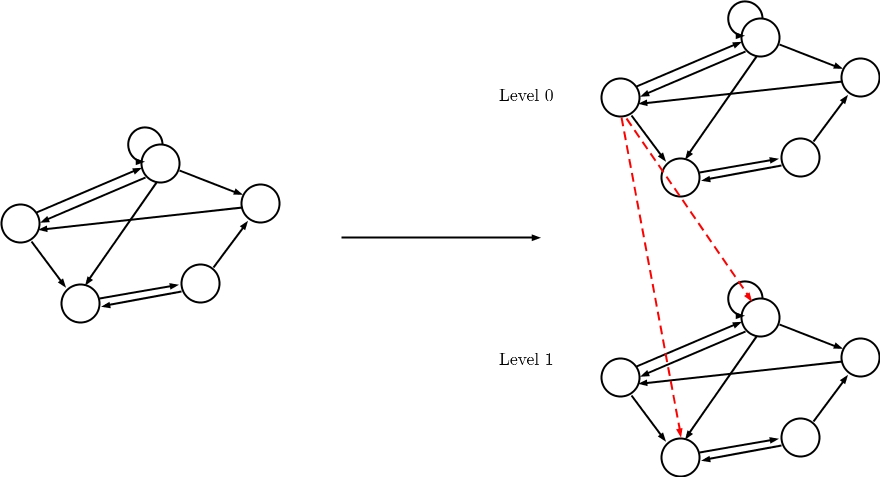
\includegraphics[width=\textwidth]{Augmented_Network}
			\caption{The original Markov Chain and the partial augmented Markov Chain}
			\label{AugNet}
		\end{figure}
		The core of the transition from state to state is a Markov Chain. Figure~\ref{AugNet} the change from a non-disruption model to a one disruption model. The important idea here is to include the record whether the disruption has happened. This means expanding the previous Markov Chain, which can be considered a network of states, to a set of networks connected by the transitions that describe disruptions. Augmenting the state space, which serves for this purpose, is equivalent to adding the red arcs in the figure. While adding all the connections between two levels, the transition probability will also change into the ones mentioned above. For the simplicity of the illustration, we only added two arcs from one node on the left. The same principle will be applied to other nodes. 
	
	\subsection{Solving the MDP}
	Remained to be finished.

	\subsection{Relaxation of the assumptions}
		\subsubsection{Relaxation of the number of disruptions}
			At first we stated that in the whole timespan there is only one possible disruption. Before and after the disruption the values and the distributions of the parameters are fixed. In order to extend this to a more general level that there may be more than one disruption happening in the timespan, we can enlarge the set of values that \(i_t\) can take in the state space. Before \(i_t\) can only take binary values to indicate whether the disruption has occurred or not. Now we can extend this to a nonnegative integer set \(\{0,1,2,\dots,L\}\), \(L\) is the maximum number of disruptions that possibly happen during the timespan.  This way we expand our network into more than two levels (shown in Figure 2). A level means one disruption and each level of the network is the identical except that the last level will be absorbing level.\\
			\newline The impact of this augmentation is that the state space expands to the size \(L|\mathscr{S}|\).
		\subsubsection{Relaxation of the magnitude of the disruption}
			Suppose at every single epoch it is possible to have a disruption where the values/distributions of the parameters may change into more than one probable result. Here "more than one" is limited to a finite integer value \(N\), and we also suppose that although the results of disruptions may be different, the possible values that a disruption can lead to do not change from time to time. Therefore, we can build parallel networks in the same level. Each parallel network represents one magnitude of the same disruption. The impact of this augmentation is that the state space expands to the size \((N+1)|\mathscr{S}|\).\\
			\newline Combining this with the result of relaxing the number of disruptions, we can build a Markov Chain with multiple levels and disjoint networks within each level. Consider each network as a circle, the structure of the newly built Markov Chain can be displayed as below.
			\begin{figure}[H]
				\centering
				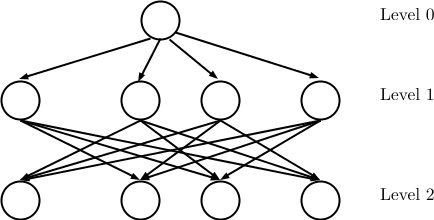
\includegraphics[width=\textwidth*3/4]{Multi_layer}
				\caption{Complete Markov Chain built from relaxations}
			\end{figure}
		\subsubsection{Relaxation of the constant probability of disruption}
			The probability for the disruption to occur may not be a constant over time. Here we would like to discuss two scenarios if the probability \(p\) is a random variable in the timespan between two disruptions. One case is that the probability is a function of time. The other one is that we have another distribution to describe the probability parameter.

	\subsection{Complexity Analysis of the MDP model}
		\cite{LDK95} systematically describes the complexity of the policy iteration algorithm and the value iteration algorithm. Suppose we have a non disruption MDP. \cite{P94} has stated that the policy iteration dominates the value iteration in the convergence rate if the discount rate is fixed. In each iteration the complexity of the policy iteration is polynomial \(O(\max(|\mathscr{S}|^2|\sup_{(s,i)} A_{(s,i)}|,|\mathscr{S}|^3))\) and the complexity of the value iteration is polynomial \(O(|\mathscr{S}|^2|\sup_{(s,i)} A_{(s,i)}|)\). \\
		\newline Therefore, the key to show that both algorithms are polynomial is to show that the value iteration algorithm can stop in polynomial number of iteration. \cite{T90} has shown this result by the following steps. First if we start from an initial value \(v_0\), the distance between \(v_0\) and the optimal value \(v^*\) is proved to be bounded given that the reward function is bounded. By the property of a contraction mapping it requires \(\log(\epsilon/\|v_0-v^*\|)/\log(\gamma)\) iterations to reach the stopping criterion \(\|v_n-v^*\|<\epsilon \quad \forall \epsilon>0\). Besides, we are able to prove that if \(\epsilon \leq \frac{1}{2\delta^{2n+2}|\mathscr{S}|^{|\mathscr{S}|}}\), the value iteration will output an optimal policy. As a result, the value iteration will have a polynomial number of iterations, thus it is a polynomial algorithm.\\
		\newline However, this proof does have the limitation as it assumes the integrality of the reward function and the fixed discount parameter.

\section{Example of the Disruption Model}\label{sec:example}
	The original non-disruption inventory problem can be found from \cite{P94} Section 3.2. With this prototype, we can come up with an example with disruptions. Consider the same company that manages the inventory of a certain product. Each time period (e.g. month) the manager needs to place an order in the beginning and will receive the order instantly (lead time is 0). 
	%The ordering decision is limited to a discrete finite sized set because of the integral unit of the product and the capacity of the facility. 
	The ordering decision is assumed to be continuous within an upper bound. A continuous-valued demand will occur through the period. If the demand exceeds the number of product on hand, each unit of shortage will be charged with a penalty price. \\
	\newline The disruption may be a result of a change in the industry, such as the upgrade of a technology, or the introduction of a new policy. The disruption will happen at the beginning of the period. There are two variations of the time when the disruption occurs. The disruption may occur before the ordering decision is made, or it can occur after the ordering decision. Both variations are realistic and the formulations are slightly different. We will mainly focus on the second variation, in which the disruption happens after the ordering decision is made.\\
	\newline   If a disruption happens, the demand, the purchase and sale prices and the inventory cost of the product are subjected to change from a fixed state to another. The scenario set is denoted by \(\Omega\), and the time of disruption \(t_d^\omega\) and the set of parameters are known for each scenario \(\omega \in \Omega\). The ordering cost contains only a variable cost. 
	%The detailed denotation of parameters of time period $t$ in scenario \(\omega\) are displayed here in Table 1. \\
	
	The timeline of the events in one epoch is shown in Figure~\ref{timeLine}. \\
	\begin{figure}[H]
		\centering
		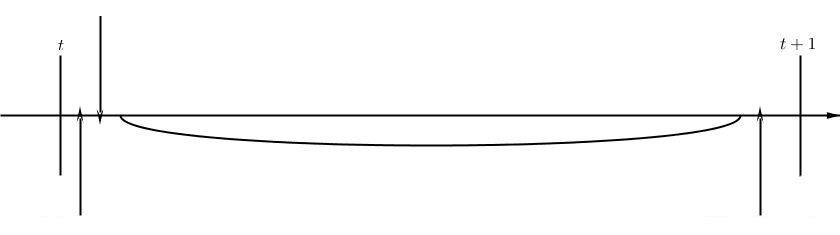
\includegraphics[width=\textwidth]{Inventory_Timeline.pdf}
		\caption{Timeline of a month}
		\label{timeLine}
	\end{figure}
	
	\subsection{Modeling the Inventory Problem with Single-Disruption with a Two-Stage Stochastic Program}
		We will introduce the stochastic programming formulation of the inventory example. Some extensions of the basic model will be included in the end of the section. 
		\begin{table}[H]
			\begin{tabular}{ l l l l }
				\\
				\multicolumn{4}{l}{Indices and index sets} \\
				\\
				\(t \in \mathscr{T}\)  & \qquad & Time periods, \(\mathscr{T} = \{1, 2 \dots T\} \text{; T is the end of the time horizon}\)& \ms \\ 
				\multirow{2}{*}{\(\omega \in \Omega\)} & \qquad & Scenarios. It contains the information of timing and extent. \\ & \qquad &This set includes the ``no-disruption scenario" denoted \(\omega_0\)& \ms\\
				\(t_d^\omega\) & \qquad & Time of disruption under scenario \(\omega\) (\(1\leq t_d^\omega \leq T\)); \(t_d^{\omega_0} = T+1\)&\\
				\\
				
				\multicolumn{4}{l}{Data} \\
				\\
				%Fixed Ordering Cost		& \(K^0\)		& \(K^1\)	\\ \hline
				\(v_t\) & \qquad & Ordering cost/unit before the disruption & \ms\\
				\(\overline{v_t^\omega}\) & \qquad & Ordering cost/unit after the disruption  & \ms\\ 
%				\(cS_t\) & \qquad & Sales price/unit before the disruption &\\
%				\(\overline{cS_t}^\omega\) & \qquad & Sales price/unit after the disruption &\\
				\(c_t\) & \qquad & Inventory cost/unit	before the disruption & \ms\\
				\(\overline{c_t^\omega}\) & \qquad & Inventory cost/unit after the disruption & \ms\\
				\(q_t\) & \qquad & Outsourcing cost/unit before the disruption & \ms\\
				\(\overline{q_t^\omega}\) & \qquad & Outsourcing cost/unit after the disruption & \ms\\ 
				\(D_t\) & \qquad & Demand set if there is no disruption, \(t \in \mathscr{T}\) & \ms\\
				\(\overline{D_t^\omega}\) & \qquad & Demand set if the disruption happens under the scenarios \(\omega\), \(t \in \{t_d^\omega, \dots, T \}\) & \ms\\ 
				\(M_t\)	& \qquad & Order capacity before the disruption & \ms\\
				\(\overline{M_t^\omega}\) & \qquad & Order capacity after the disruption & \ms\\
				\(p^\omega\) & \qquad & Probability of scenario \(\omega\) &\\
				\\
				
				\multicolumn{4}{l}{Variables} \\
				\\
				%Fixed Ordering Cost		& \(K^0\)		& \(K^1\)	\\ \hline
				\(X_t\) & \qquad & Number of units ordered in period \(t\) given the disruption has not happened in period \(t\)& \ms\\
				\(Q_t\) & \qquad & Number of units outsourced in period \(t\) given the disruption has not happened in period \(t\)& \ms\\
				\(I_t\) & \qquad & Inventory in period \(t\) given the disruption has not happened in period \(t\)& \ms\\
				\(\overline{X_t^\omega}\) & \qquad & Number of units ordered in period \(t\) given the disruption has happened before the end of period \(t\)& \ms\\
				\multirow{2}{*}{\(\overline{Q_t^\omega}\)} & \qquad & Number of units outsourced in period \(t\) given the disruption has happened before \\ & \qquad & the end of period \(t\)& \ms\\
				\(\overline{I_t^\omega}\) & \qquad & Inventory in period \(t\) given the disruption has happened before the end of period \(t\)& \ms\\
			\end{tabular}
		\end{table}
		
		\noi The two stage stochastic linear programming can be formulated as follows, \(I_0\) is a constant and we force \(\overline{v^\omega_{t_d^\omega}} = v_{t_d^\omega}, \forall \omega \in \Omega\).
		\begin{align*}
			 \min \quad & \sum_{\omega \in \Omega} p^\omega [\sum_{t = 1}^{t_d^\omega-1}{(c_tI_t + v_tX_t + q_tQ_t)} + \sum_{t = t_d^\omega}^{T}{(\overline{c_t^\omega}\ \overline{I_t^\omega} + \overline{v_t^\omega}\ \overline{X_t^\omega} + \overline{q_t^\omega}\ \overline{Q_t^\omega})}] & \\
			 \text{s.t.} \quad & I_{t-1} + X_{t} - D_{t} + Q_{t} = I_{t} & \forall t = 1, \dots, T\\
			& \overline{I_{t-1}^\omega} + \overline{X_{t}^\omega} - \overline{D_{t}^\omega} + \overline{Q_{t}^\omega} = \overline{I_{t}^\omega} \qquad \forall t = t_d^\omega, \dots, T, & \forall \omega \in \Omega \\
			& I_{t_d^\omega-1} = \overline{I_{t_d^\omega -1}^\omega} & \forall \omega \in \Omega \\
			& X_{t_d^\omega} = \overline{X_{t_d^\omega}^\omega} & \forall \omega \in \Omega \\
			& X_t \leq M_t & \forall t = 1, \dots, T\\
			& \overline{X_{t}^\omega} \leq \overline{M_t^\omega} & \forall t = t_d^\omega, \dots, T, \  \forall \omega \in \Omega\\
			& X, I, Q, \overline{X^\omega}, \overline{I^\omega}, \overline{Q^\omega} \geq 0. &
		\end{align*}
		\noi The master program is displayed as follows. Since the problem has a relatively complete recourse, we do not need to generate feasibility cuts. The optimality cuts use the \(k^{\text{th}}\) optimal dual variables of the constraints in the subproblem.
		\begin{align*}
		\min \quad & \sum_{\omega \in \Omega} p^\omega \sum_{t = 1}^{t_d^\omega - 1} (c_t I_t + v_t X_t + q_t Q_t) + p^\omega \phi_\omega & \\
		\text{s.t.} \quad & I_{t-1} + X_t - D_t + Q_t = I_t \quad & \forall t = 1, \dots, T \\
		& X_t \leq M_t & \forall t = 1, \dots, T \\
		& \phi_\omega \geq \mathcal{G}\omega(I_{t_d^\omega - 1}^k,X_{t_d^\omega}^k) + \pi_{I,\omega}^k (I_{t_d^\omega - 1} - I_{t_d^\omega - 1}^k) + \pi_{X,\omega}^k (X_{t_d^\omega} - I_{t_d^\omega}^k) & \forall k = 1,2, \dots\\
		& X,I,Q \geq 0 & 
		\end{align*}
		\noi The subprogram for a specific scenario \(\omega \in \Omega\) is denoted as \(\mathcal{G}_\omega(I_{t_d^\omega - 1},X_{t_d^\omega})\).
		\begin{align*}
			\mathcal{G}(I_{t_d^\omega - 1},X_{t_d^\omega}) = \min \quad & \sum_{t = t_d^\omega}^{T} (\overline{c_t^\omega} \overline{I_t^\omega} + \overline{v_t^\omega} \overline{X_t^\omega} + \overline{q_t^\omega} \overline{Q_t^\omega}) &\\
			\text{s.t.} \quad & \overline{I_{t-1}^\omega} + \overline{X_t^\omega} - \overline{D_t^\omega} + \overline{Q_t^\omega} = \overline{I_t^\omega}, & \forall t = t_d^\omega, \dots, T \qquad :\gamma_t\\
			& \overline{I_{t_d^\omega -1}^\omega} = I_{t_d^\omega - 1} & \qquad : \pi_I \\
			& \overline{X_{t_d^\omega}^\omega} = I_{t_d^\omega} & \qquad : \pi_X \\
			& \overline{X_t^\omega} \leq \overline{M_t^\omega} & \forall t = t_d^\omega, \dots, T \qquad: u_t
		\end{align*}
		
	\subsection{Modeling the Inventory Problem with Multiple-Disruptions with a Multi-Stage Stochastic Program}
	Remained to be finished.
		
	\subsection{Example: Modeling the Inventory Problem with MDP}
		For the example in section~\ref{sec:example}, the unit of the decision epoch is one month. \[\mathscr{T}=\{1,2,\dots,T_{max}\}, \quad T_{max}\leq +\infty\]
		The state of this problem is the tuple that consists of the inventory on hand at the beginning of each decision epoch and the binary variable indicating whether the disruption has happened. It is realistic to suppose the inventory is integer and has an upper bound \(M\). Then the state space of the problem is \[\mathscr{S}=\{(0,0),(1,0),\dots,(M,0),(0,1),(1,1),\dots,(M,1)\}\]
		Suppose at the beginning of the epoch \(t\) the state is \((s_t,i_t),  s_t \in \mathbb{Z}^+, s \leq M, i_t \in \{0,1\}\). The action means the number of the product to be purchased in epoch \(t\). Therefore, the action space is an integer set with an upper bound \(M-s_t\). \[A_{(s_t,i_t)}=\{0, 1, \dots, M-s_t\}\]
		The calculation for the expected reward of each epoch can be divided into three parts: the ordering cost, the holding cost and the revenue. The ordering cost is a function of the action and can be calculated with the following equation. \[O((s_t,i_t),a) = \begin{cases}
		K^i+c_v^{i_t}a & \text{if } a \geq 0 \\
		0 & \text{if } a = 0
		\end{cases}
		\qquad a \in A_{(s_t,i_t)}\]
		The holding cost \(h((s_t,i_t))\) is proportional to the number of products the factory holds for epoch \(t\). According to the timeline in Section 1.2, the number of products held in the inventory is the state at the beginning of epoch \(t\), \(s_t\). Therefore, \[h((s_t,i_t),a)=c_I^{i_t}s_t\]
		It takes more than just the current state to calculate the revenue as the revenue depends on both the current state and the demand information. However, the demand information is stochastic. To express this deterministically, the way in Puternam is to calculate the revenue using both the current state \(s_t\) and the next epoch's state \(s_{t+1}\). \[R((s_t,i_t),(s_{t+1},i_{t+1}),a)=c_s^{i_t}(s_{t+1}-(s_{t}+a))\] 
		This is an exact way to express the revenue, but later we will derive the optimality equation for this MDP and the dependence on the next epoch's state will disappear when we take the expectation value. The expected revenue does not depend on exact demand occurring in this epoch, but depends on the distribution of the demand only. Suppose the probability if a demand \(d\) occurs is denoted by \(p^{*i_t}_d\). The expected revenue is \[R_E((s_t,i_t),a)=c_s^{i_t}(\sum_{d \in D^{i_t}}p^{*i_t}_{d|s_t}d)\]
		The transition probability matrix could be formed if we are given with a specific policy \(\pi=(\delta^1,\delta^2,\dots)\), just as stated in Section 2.1. The transition probability from the state \((s_t,i_t)\) to \((s_{t+1},i_t)\) is \[ Pr\{(s_{t+1}i,_{t+1})|(s_t,i_t),\delta_{(s_t,i_t)}\} = \begin{cases} 
		p^{*i_t}_{s_t+a-s_{t+1}}(1-p) & \quad \text{if } s_{t+1} \neq 0, i_t = 0, i_{t+1} = 0\\ 
		\sum_{d \geq s_t+a} p^{*i_t}_d(1-p) & \quad \text{if } s_{t+1} = 0, i_t=0, i_{t+1} = 0\\ 
		p^{*i_t}_{s_t+a-s_{t+1}}p & \quad \text{if } s_{t+1} \neq 0, i_t = 0, i_{t+1} = 1\\ 
		\sum_{d \geq s_t+a} p^{*i_t}_dp & \quad \text{if } s_{t+1} = 0, i_t=0, i_{t+1} = 1\\ 
		p^{*i_t}_{s_t+a-s_{t+1}} & \quad \text{if } s_{t+1} \neq 0, i_t = 1, i_{t+1} = 1\\ 
		\sum_{d \geq s_t+a} p^{*i_t}_d & \quad \text{if } s_{t+1} = 0, i_t=1, i_{t+1} = 1\\ 
		0 & \quad \text{Otherwise}
		\end{cases} \]

	
\section{Comments}
Remained to be finished.
	
\section{Other thoughts}
Remained to be finished.

%----------------------------------------------------------------------------------------------------------------------
\bibliographystyle{plain}
\bibliography{disruption}
%----------------------------------------------------------------------------------------------------------------------
	
\end{document}


%	With the formulation in the section 1, if we assume each change can only be binary and the possibility of change is known to us as \(p\), then we can rewrite the problem as:
%	\begin{align*}
%	\min \quad & C_Tx+\sum_{i=1}^Tp_ih_i(x_1,\dots,x_i)\\
%	\text{s.t.} \quad & Dx \leq d\\
%	& x \geq 0
%	\end{align*}
%	If we can assume that the problem \(h(x_1,\dots,x_i)\) is a linear programming problem which can be rewritten as:
%	\begin{align*}
%	h(x_1,\dots,x_i)= \min \quad & q_iy_i \\
%	\text{s.t.} \quad & B_ix+D_iy_i=d_i\\
%	\end{align*}
%	Here we let \(h_T(x_1,\dots,x_T)=0\). We may use \(\theta_i\) to create cut for each scenario and each scenario is corresponding to the stage of the disruption happening.
	
%	After the change, if the part of \(h_i(x_1,\dots,x_i)\) corresponding to each time period has the same form and is independent from each other, we can rewrite the problem in the following form. Here we use an example of resource allocation problem. Suppose we use \(x\) as the capacity we invest in, we would like to minimize the total cost of the entire plan. If we assume each time period the decisions are independent, function \(h_i\) will be equivalent to optimizing over a single time period:
%	\begin{align*}
%	\min \quad & \sum_{j=1}^m C^Y_jy_j\\
%	\text{s.t.} \quad & \sum_{j=1}^m y_j \leq \sum_{\tau=1}^i x_{\tau}
%	\end{align*}
%	The whole formulation will turn to, if we do not consider the discount factor, the following program:
%	\begin{align*}
%	\min \quad & \sum_{i=1}^T (1-p)^{i-1}(C_ix_i+p(T+1-i)\min \sum_{j=1}^m C^Y_jy_{ij})\\
%	\text{s.t.} \quad & \sum_{j=1}^m y_{ij} \leq \sum_{\tau=1}^i x_\tau \quad \forall i=1 \dots T\\
%	& Dx \leq d\\
%	& x \geq 0
%	\end{align*}

% Whatever might be useful...

% \begin{equation}\label{model:true}
 
% \end{equation}

% \begin{subequations}
% \begin{eqnarray}
% \P \left [ \sqrt{n} \left ( L_n(\theta_n^*) - z^* \right ) \le \eta s_{\max}  \right ]  & \ge &\dst  \P \left [  \sqrt{n} \left ( \bar{F}_{N_k}(\theta^*) - z^* % \right )/\sigma(\theta^*) \le \eta \left ( \frac{s_{\max}}{\sigma(\theta^*)} \right)  \, : \, \forall k \right ] \\
% & = & \dst  \left ( \P \left [  \sqrt{n} \left ( \bar{F}_{N_k}(\theta^*) - z^* \right ) / \sigma(\theta^*) \le \eta  \left ( \frac{s_{\max}}{\sigma(\theta^*)} \right)   \right ] \right )^K,
% \end{eqnarray}
% \end{subequations}

% \begin{theorem}\label{the_lb_theorem}
% Consider model~~\eqref{model:true}, where $\Theta \neq \emptyset$ is convex, $F(\cdot,x,y)$ is convex for all $(x,y)$, $\var [ F(\theta,x,y) ] < \infty$ for all $\theta \in \Theta$, and $z^* > -\infty$. Let $(x^i,y^i)$, $i=1,2,\ldots$ be i.i.d.\ observations partitioned into non-overlapping batches indexed by $N_k$, $k=1,2,\ldots,K$, where $|N_k|=n$ for all $k$. Define $s^2_{\max}$ as in equations~\eqref{sample_variance} and~\eqref{eqn:smax}. Let $0 < \alpha < 1/2$, define $\eta_\ell$ via $\P \left [ \cN(0,1)  \le \eta_\ell \right ] = (1-\alpha)^{1/K}$, and let $L_n(\theta_n^*)$ be the optimal value of~\eqref{eqn:LP}. Assume $\liminf_{n \rightarrow \infty} s^2_{\max} \ge \inf_{\theta \in \Theta^*} \var [ F(\theta,x,y) ]$, w.p.1., where $\Theta^*$ is the set of optimal solutions to~\eqref{model:true}, e.g., a singleton set if~\eqref{model:true} has a unique optimal solution. Then,
% \begin{equation}\label{eqn:lower_bound_result}
% \liminf_{n \rightarrow \infty} \P \left [  L_n(\theta_n^*) - \frac{\eta_\ell s_{\max}}{\sqrt{n}} \le  z^*\right ]  \ge  1-\alpha.
% \end{equation}
% \end{theorem}
